\documentclass[10pt,pdftex]{report}
\usepackage[T1]{fontenc}
\usepackage[utf8]{inputenc}
\usepackage[magyar]{babel}
\usepackage{graphicx}
\usepackage{amsmath}
\usepackage{amssymb}
\usepackage{multirow}
\usepackage{booktabs}
\usepackage{indentfirst}
\usepackage[a4paper]{geometry}
\usepackage{url}
\usepackage{titling}
\usepackage{float}
\usepackage{spverbatim}
\usepackage{xcolor}
\usepackage{hyperref}
\usepackage{svg}
\usepackage{subcaption}
\usepackage{adjustbox}
    \definecolor{titlebg}{RGB}{128,128,128}

\usepackage{lmodern}
\usepackage{etoolbox}
\patchcmd{\thebibliography}{\chapter*}{\section*}{}{}

\renewcommand{\thesection}{\arabic{section}}


\title{Egyszerű mozgások vizsgálata}

%% EZ ALÁBBI KÉT MEZŐT ÉRTELEMSZERŰEN KI KELL TÖLTENI
\author{Bíró Gergő Tamás}
\date{2025. április 1.}


%% FEJLÉC LEÍRÓ, NEM KELL MÓDOSÍTANI
\renewcommand*{\maketitle}{\noindent{%
\parbox{\dimexpr\linewidth-2\fboxsep}{\color{black}%
\parbox{\linewidth}{\fontsize{18}{24}\selectfont\sffamily\bfseries\thetitle}%
}}\vskip 1em%
\begin{tabular}{l}%
Mérést végezte: \theauthor \\%
Mérés dátuma: \thedate\\
Jegyzőkönyv végleges változata: \today \\%
Jegyzőkönyv leadásának időpontja: 2025. április 8.
\end{tabular}%
}
%%%%%%%%%%%%%%%%%%%%%

\begin{document}
\maketitle
\section*{Mérés célja}
A Mikola-csövön végzett mérések során igazolni szeretnénk, hogy a csőben a buborék jó közelítessel végig egyenes vonalú egyenletes mozgást végez, emellett még a buborék sebességének a cső dőlésszögétől való függését is meg akarjuk vizsgálni. A második mérés során pedig a nehézségi gyorsulás nagyságát, és annak a hibáját szeretnénk meghatározni, és igazoljuk a szabadeső test mozgását leíró $s=\frac{g}{2}t^2$ egyenletet, ahol $g$ a nehézségi gyorsulás, $s$ az ejtés magassága és $t$ a test szabadesésének ideje.
\section*{Mérőeszközök}
\begin{itemize}
    \item{Mikola-cső}
    \item{Mikola program, amellyel az időt mérjük, és a sebeségeket határozzuk meg.}
    \item{Elektronikus óra}
    \item{Mágneses indítószerkezet}
    \item{Skálázott acélrúd, melyen az indítószerkezet magasságát állíthatjuk.}
    \item{Fémgolyó}
\end{itemize}
\section*{A mérés leírása}
\subsection*{Buborék mozgásának vizsgálata}
A Mikola-csövet a megadottdőlésszögekbe beállítjuk, majd a buborékot az üvegcső végén lévő hajlítható műanyagcső kiegyenesítésével elindítjuk. A Mikola program segítségével rögzítjük a mozgás során eltelt időt, amikor a buborék a csövön lévő 0, 15, 30, 45, 60, 75 és 90cm-nél elhelyezkedő jelöléseket eléri, ezeket az időket később mi is feljegyezzük. A prtogram az egyes mérések végeztével az előre megadott távolságokra egyenest illeszt, amelyek meredeksége a buborék sebességét adja meg $cm/s$-ban, ezeket a sebességértékeket és az illesztések pontosságát leíró 0 és 1 közötti számokat fejegyezzük. Ezen kívül még a buborékok alakját is megfigyeljük $10^{\circ}$, $45^{\circ}$, valamint $90^{\circ}$-os szögek mellett.
\subsection*{Nehézségi gyorsulás mérése}
A méréshez először az indítószerkezet 10cm magasra emeljük a rúdon, a fémgolyót az indítószerkezetbe helyezzük, ahol egy mágnes fogja megtartani az indításig. Az órának ekkor vissza kell állnia 0s-ra, mivel a fém zárni fogja az ezért felelős áramkört. Azonban ez nem midig történik meg a fém felületén lévő szennyződések miatt, ekkor a golyó kis mértékű mozgatásával tudjuk elérni az áramkör záródását. Ezután az indítószerkezet tetején található gomb megnyomásával a mágnes elemelhkedik a golyótól, ami emiatt leesik. Ekkor az óra is elkezdi mérni az időt, mivel az áramkör már nem lesz zárva. Az óra akkor áll meg, amikor a golyó eléri az állvány talpát, és azt egy szenzor érzékeli. Az ekkor az órán látható időt leolvassuk, és feljegyezzük. Ezt még kétszer megismételjük ezen a magasságon. Ezután az indítás magasságát 5cm-el megnöveljük, és az előzőleg leírt mérést végezzük el ismét addig amíg az ejtés magassága nem haladja meg a 95cm-t.
\section*{Mérési adatok}
\subsection*{Buborék mozgásának vizsgálata}
\begin{table}[H]
    \centering
    \begin{tabular}{|r|r|r|r|r|r|r|r|}
        \hline
        \multirow[c]{3}{*}{$távolság(m)$} & \multicolumn{7}{|c|}{$Hajlásszög(^{\circ})$} \\
        \cline{2-8}
        & 10 & 20 & 40 & 45 & 50 & 70 & 90 \\
        \cline{2-8}
        & \multicolumn{7}{|c|}{$idő(s)$} \\
        \hline
        0.00 & 0.000 & 0.000 & 0.000 & 0.000 & 0.000 & 0.000 & 0.000 \\
        \hline
        0.15 & 5.093 & 3.752 & 3.138 & 3.065 & 3.096 & 4.349 & 5.475 \\
        \hline
        0.30 & 10.628 & 8.022 & 6.344 & 6.376 & 6.504 & 8.691 & 11.428 \\
        \hline
        0.45 & 15.682 & 12.036 & 9.610 & 9.577 & 9.632 & 12.992 & 17.102 \\
        \hline
        0.60 & 20.974 & 16.169 & 12.856 & 12.928 & 12.944 & 17.549 & 23.039 \\
        \hline
        0.75 & 26.385 & 20.278 & 16.114 & 16.176 & 16.272 & 21.970 & 28.921 \\
        \hline
        0.90 & 31.748 & 24.365 & 19.402 & 19.400 & 19.662 & 26.518 & 34.976 \\
        \hline
    \end{tabular}
    \caption{Az egyes távolságok elérésének ideje a szögtől függően.}
\end{table}
\begin{table}[H]
    \centering
    \begin{tabular}{|r|r|r|r|r|r|r|r|}
        \hline
        & \multicolumn{7}{|c|}{$Hajlásszög(^{\circ})$} \\
        \hline
        $sebesség\left(\frac{m}{s}\right)$ & 0.02834 & 0.03674 & 0.04632 & 0.04616 & 0.04576 & 0.03396 & 0.02570 \\
        \hline
        R\footnotemark & 1.0000 & 0.9999 & 1.0000 & 1.0000 & 0.9999 & 1.0000 & 0.9999 \\
        \hline
    \end{tabular}
    \caption{A sebességek, és az adatokva való egyenes illesztésének pontossága a szög függvényében.}
\end{table}
\footnotetext{R az egyenesillesztés pontosságát megadó 0 és egy közötti szám, minél közelebb van az értéke 1-hez az illesztés annál pontosabb.}
\subsection*{Gravitációs gyorsulás vizsgálata ejtőgéppel}
\begin{table}[H]
    \centering
    \begin{tabular}{|r|r|r|r|r|}
        \hline
        \multirow[c]{2}{*}{$magasság(m)$} & \multicolumn{4}{|c|}{$esés ideje(s)$} \\
        \cline{2-5}
        & 1. & 2. & 3. & Átlag \\
        \hline
        0.10 & 0.155 & 0.153 & 0.147 & 0.1517 \\
        \hline
        0.15 & 0.181 & 0.180 & 0.181 & 0.1807 \\
        \hline
        0.20 & 0.203 & 0.210 & 0.207 & 0.2067 \\
        \hline
        0.25 & 0.230 & 0.225 & 0.229 & 0.2280 \\
        \hline
        0.30 & 0.248 & 0.263 & 0.257 & 0.2560 \\
        \hline
        0.35 & 0.272 & 0.270 & 0.272 & 0.2713 \\
        \hline
        0.40 & 0.286 & 0.286 & 0.296 & 0.2893 \\
        \hline
        0.45 & 0.306 & 0.303 & 0.304 & 0.3043 \\
        \hline
        0.50 & 0.321 & 0.320 & 0.319 & 0.3200 \\
        \hline
        0.55 & 0.335 & 0.337 & 0.342 & 0.3380 \\
        \hline
        0.60 & 0.350 & 0.353 & 0.353 & 0.3520 \\
        \hline
        0.65 & 0.369 & 0.367 & 0.370 & 0.3687 \\
        \hline
        0.70 & 0.382 & 0.382 & 0.381 & 0.3817 \\
        \hline
        0.75 & 0.396 & 0.398 & 0.403 & 0.3990 \\
        \hline
        0.80 & 0.407 & 0.412 & 0.408 & 0.4090 \\
        \hline
        0.85 & 0.417 & 0.420 & 0.426 & 0.4210 \\
        \hline
        0.90 & 0.435 & 0.436 & 0.432 & 0.4343 \\
        \hline
        0.95 & 0.443 & 0.445 & 0.445 & 0.4443 \\
        \hline
    \end{tabular}
    \caption{Esések ideje adott magasságokon.}
\end{table}
\section*{Hibaforrások}
A Mikola-csövön végzett mérés során:
\begin{enumerate}
    \item{A hajlásszög nem egyezik meg pontosan a megadott értékkel, mivel az ezért felelős mechanizmus néhány fokkal el tud fordulni, mivel nem elég szoros.}
    \item{A csövön lévő skála nem biztos, hogy teljesen pontos, az egyes beosztások néhány miliméterrel eltérhetnek attól ahol lenniük kéne.}
    \item{Az emberi szem pontatlansága és az emberi reakcióidő miatt az idő nem a megfelelő időpillanatban lesz rögzítve.}
    \item{A buborék nem biztos, hogy eléri a végleges sebességig addig, amíg eléri a mérés során 0-nak választott távolságot, így a mozgás elején még minimálisan gyorsulhat.}
\end{enumerate}


A szabadesés vizsgálata során:
\begin{enumerate}
    \item{A skála pontatlansága miatt az ejtés magassága nem fog teljesen megegyezni a megadott magasságokkal.}
    \item{Az indítás során az állvány és a rúd megmozdulhat, emiatt a golyónak lehet egy kis méretű kezdősebessége.}
    \item{Az óra nem pontosan akkor áll le, amikor a golyó eléri a talpat, mivel a szenzor egy kis mértékű késést visz a rendszerbe.}
\end{enumerate}
\section*{A mérés kiértékelése}
\subsection*{Buborék mozgásának vizsgálata Mikola-csőben}
A buborék mozgása során mért idők függvényében ábrázolva a távolságokat a következő ábrát kaphatjuk:
\begin{figure}[H]
    \centering
    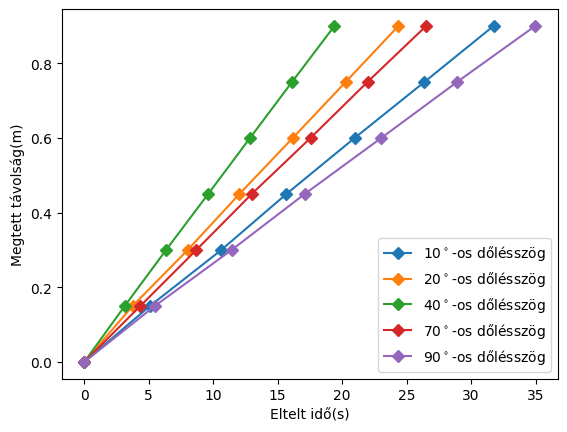
\includegraphics{./mikola_ut-ido.png}
    \caption{A buborék mozgásának út-idő grafikonja különböző dőlésszögeknél.}
\end{figure}
A fenti ábrán a $45^{\circ}$ és a $50^{\circ}$-os dőlésszögeknél végzett mérések adatai nincsenek ábrázolva, mivel az azokhoz tartozó adatok csak kis mértékben térnek el a $40^{\circ}$-os esettől, így rosszul lehetne őket látni. A buborék sebességét az egyes szögek mellett a Mikola program határozta meg az út-idő grafikonra illesztett egyenes meredekségéből, amely a jelenlegi vizsgálatunkhoz kellően pontos, mivel a korrelációs együttható értéke minden esetben nagyon közel van az 1-hez. A sebességeket a dőlésszög függvényében ábrázolva a következő ábrát kapjuk:
\begin{figure}[H]
    \centering
    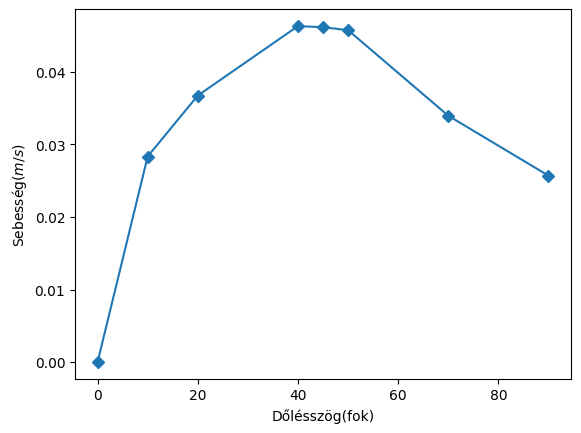
\includegraphics{./mikola_sebessegek.png}
    \caption{A buborék mozgásának sebessége a dőlésszög függvényében.}
\end{figure}
Ezen az ábrán a mért adatsorhoz még hozzáadtuk a $0^{\circ}$-hoz tartozó esetet, amelyben a buborék sebessége $0\frac{m}{s}$, hiszen csak a csőre merőleges komponensű erők fognak rá hatni, így nem fog elkezdeni mozogni. A buborék mozgását két erő befolyásolja lelentős mértékben: a közegellenállás és a felhajtóerő a csővel párhuzamos komponense. A felhajtóerő nagysága állandó a szög függvényében, hiszen a buborék térfogata jó közelítéssel állandó, azonban a cső irányú komponense a szög növelésével nő, ám a buborék alakja és keretmetszetének a felülete nem lesz független a dőlésszögtől, így a közegellenállás függeni fog a szögtől. Emiatt alakul ki a fenti ábrán is látható sebességfüggése a sebességnek, amelynek nagysága $40^{\circ}$ körül a legnagyobb, $90^{\circ}$-nál pedig már valamivel kisebb is mint $10^{\circ}$-nál. A buborék alakját és keresztmetszetét legfőképpen a felületi feszültség befolyásolja. A $10^{\circ}$, $45^{\circ}$ és $90^{\circ}$ mellett a buborékok alakjának vázlatos rajazai a következők:
\begin{figure}[H]
    \centering
    \begin{subfigure}{0.33\textwidth}
        \centering
        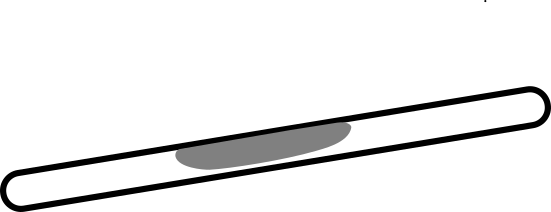
\includegraphics[width=1\linewidth]{./10_fok.png}
        \caption{A buborék alakja $10^{\circ}$-os dőlésszög mellett.}
    \end{subfigure}
    \begin{subfigure}{0.33\textwidth}
        \centering
        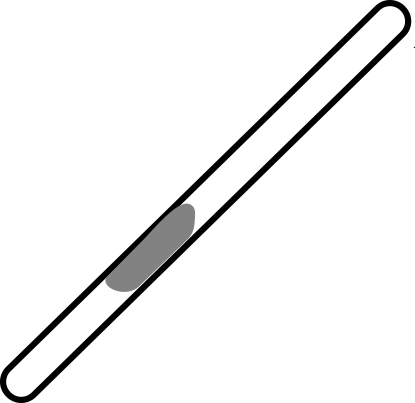
\includegraphics[width=1\linewidth]{./45_fok.png}
        \caption{A buborék alakja $45^{\circ}$-os dőlésszög mellett.}
    \end{subfigure}
    \begin{subfigure}{0.33\textwidth}
        \centering
        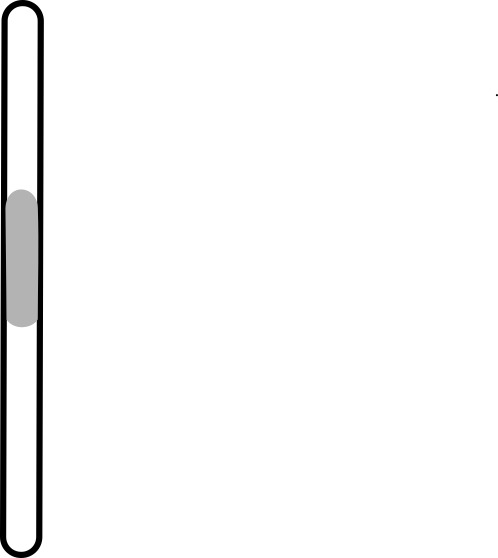
\includegraphics[width=1\linewidth]{./90_fok.png}
        \caption{A buborék alakja $90^{\circ}$-os dőlésszög mellett.}
    \end{subfigure}
    \caption{A buborék vázlatos rajza különböző dőlésszögek mellett.}
\end{figure}
A sebességnek a nagysága abban a szögben lesz a legnagyobb, ahol a felhajtóerő csőre párhuzamos komponensének és a közegellenállási együtthatónak az aránya a legnagyobb, amely jelen esetben $40^{\circ}$ körül valósulhat meg.
\subsection*{A nehézségi gyorsulás mérése}
A mérés során használt magasságokat a hozzájuk tartozó átlagidő függvényében ábrázoljuk, a kapott rafikonra illesszünk $y=mx+b$ alakú függvény, amelyben lejen esetben $y=s$ vagyis az ejtés magassága, $x=t^2$ az átlagidő négyzete és $m=\frac{g}{2}$ a negézségi gyorsulás fele. Várhatóan mivel a kezdősebesség 0, és a gravitáción kíbül minden más erő szinte teljesen elhanyagolható $b$ értékének jó közelítéssel 0-nak kell lennie.
\begin{figure}[H]
    \centering
    \begin{subfigure}{\textwidth}
        \centering
        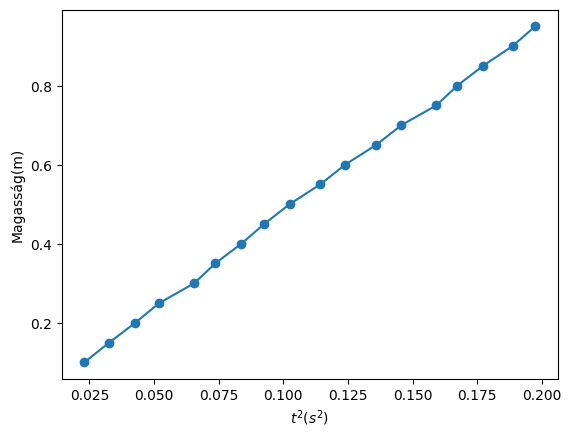
\includegraphics[width=0.5\linewidth]{./szabadeses_adatok.png}
        \caption{A mérés során kapott adatok.}
    \end{subfigure}
    \begin{subfigure}{\textwidth}
        \centering
        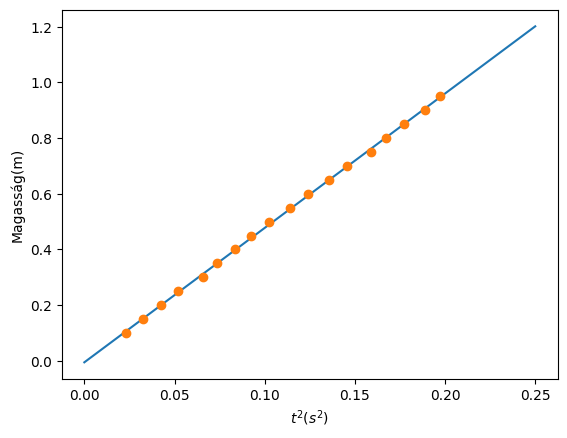
\includegraphics[width=0.5\linewidth]{./szabadeses_illesztes.png}
        \caption{A mért adatok és az illesztett egyenes.}
    \end{subfigure}
    \caption{A magasságok az idő négyzetének a föggvényében.}
\end{figure}
Az illesztés pythonban a scipy.optimize modul curve\_fit függvényével lett elvégezve, $m=4.824$ és $b=-0.0051$ adódik, tehát az egyenes egyenlete $y=4.824x-0.0051$. A vártaknak megfelelően $b$ tényleg közel 0, $g$ értéke pedig $g=2m=9.6495\frac{m}{s^2}$.
Az az illesztett egyenes meredekségének hibáját a téglalap módszerrel határozzuk meg, ehhez legyen $y_{ill}$ az illesztés során kapott egyenes adott $x$ mellett felvett értéke, és $\Delta y=y-y_{ill}$. $x=t^2$, $y$, $y_{ill}$ és $\Delta y$ értékei a következők:
\begin{table}[H]
    \centering
    \begin{tabular}{|r|r|r|r|}
        \hline
        $x=t^2(s^2)$ & $y(m)$ & $y_{ill}(m)$ & $\Delta y(m)$ \\
        \hline
        0.0230 & 0.10 & 0.1059 & -0.00586 \\
        \hline
        0.0326 & 0.15 & 0.1524 & -0.00236 \\
        \hline
        0.0427 & 0.20 & 0.2009 & -0.00095 \\
        \hline
        0.0520 & 0.25 & 0.2457 & 0.00431 \\
        \hline
        0.0656 & 0.30 & 0.3111 & -0.01107 \\
        \hline
        0.0736 & 0.35 & 0.3501 & -8.41$\cdot10^{-5}$ \\
        \hline
        0.0837 & 0.40 & 0.3988 & 0.00122 \\
        \hline
        0.0926 & 0.45 & 0.4417 & 0.00826 \\
        \hline
        0.1024 & 0.50 & 0.4889 & 0.01107 \\
        \hline
        0.1142 & 0.55 & 0.5461 & 0.00392 \\
        \hline
        0.1239 & 0.60 & 0.5927 & 0.00732 \\
        \hline
        0.1359 & 0.65 & 0.6506 & -0.00063 \\
        \hline
        0.1457 & 0.70 & 0.6977 & 0.00230 \\
        \hline
        0.1592 & 0.75 & 0.7623 & -0.01298 \\
        \hline
        0.1673 & 0.80 & 0.8020 & -0.00197 \\
        \hline
        0.1772 & 0.85 & 0.8500 & -2.10$\cdot10^{-5}$ \\
        \hline
        0.1886 & 0.90 & 0.9050 & -0.00504 \\
        \hline
        0.1974 & 0.95 & 0.9474 & 0.00256 \\
        \hline
    \end{tabular}
    \caption{$\Delta y$, $y$ és $y_{ill}$ értékei $t^2$ értékei mellett.}
\end{table}
A meredekségre vonatkozó hibaszábítás:
\begin{equation*}
    \Delta m = 2\frac{\left|\Delta y\right|_{max}}{x_{max}-x_{min}}=2*\frac{0.01298}{0.1974-0.0230}=0.0744
\end{equation*}
Tehát $\Delta g=2\Delta m=0.1488\frac{m}{s^2}$.
\begin{table}[H]
    \centering
    \begin{tabular}{|r|r|r|}
        \hline
        Meggyiség & Mérésből kapott érték hibával & Irodalmi érték \\
        \hline
        $g$ & $9.6495\pm0.1488\frac{m}{s^2}$ & $9.81\frac{m}{s^2}$ \\
        \hline
    \end{tabular}
    \caption{A mérésből kapott érték.}
\end{table}
\section*{Diszkusszió}
A mérési eredményekből jól látható az, hogy a Mikola-csőben a buborék tényleg egyenes vonalú, egyenlertes mozgást végez, valamint sikerült kvalitatívan magyarázni a sebességének a dőlésszögtől való függését. A szabadesés vizsgálata során sukerült igazolni a test mozgását leíró egyenletet, mivel abban elhanyagolható mértékű volt az illesztés során kapott konstans, az egyenes nagy pontossággal illeszkedett a mért adatokra. A nehézségi gyorsulás meghatározása is sikeres volt, értéke habár nincs hibahatáron belül az irodalm értékéhez képest attól csak nagyon kis mértékben tér el, és ha pontosabb hibaszámítási modellt alkalmaznánk, akkor már feltehetőleg hibahatáron belül lenne az általunk mért érték.
\end{document}

%rúd téglalap